\section{Aplicación móvil}

Un completo análisis para el desarrollo de la aplicación móvil se incluye en un capítulo posterior de este documento (\ref{part:analisisAplicacion}). Esta sección pretende mostrar los resultados de la implementación realizada. \\

La aplicación permitirá al usuario registrar ciertos datos de los pacientes, incluyendo el número telefónico asociado a la tarjeta SIM ubicada en el módulo 4G. Una vez registrado un usuario, podrá consultar y editar esta información. \\

Al consultar los registros de los signos vitales, se recuperará la información de los mensajes de texto y de la base de datos para mostrar la información actualizada de estas mediciones. \\

Estas funcionalidades se muestran en la figura \ref{fig:casosUso:AplicacionResumen}

\begin{figure}[htpb!]
	\begin{center}
		\fbox{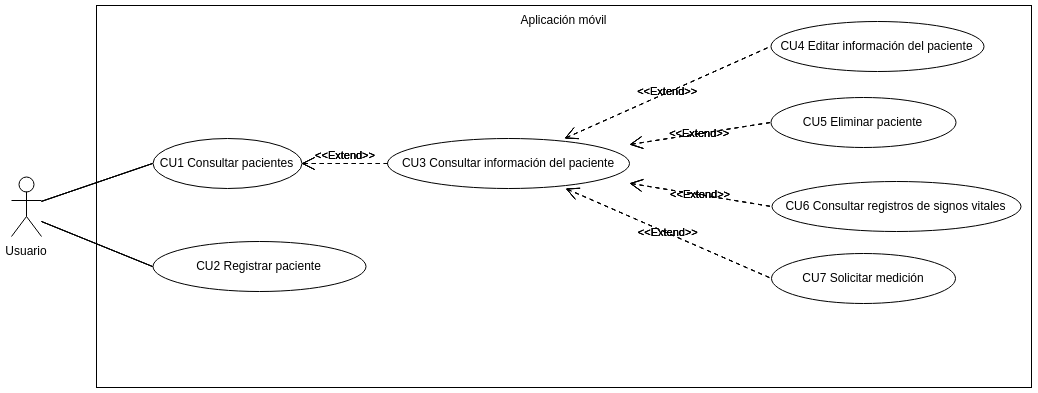
\includegraphics[width=1\textwidth]{ModeloComportamiento/imagenes/CasosUso_Usuario.png}}
		\caption{Diagrama de casos de uso del módulo Aplicación Móvil. \label{fig:casosUso:AplicacionResumen}}
	\end{center}
\end{figure}

\subsection{Diseño de pantallas}

La aplicación móvil consta de 5 pantallas principales que permiten realizar alguna funcionalidad de la aplicación y sobre las que se muestran mensajes emergentes con información para el usuario. \\


\subsubsection{IU Consultar pacientes}
La figura \ref{fig:casosUso:resumenUI1} muestra la pantalla ''Consultar pacientes'' en la que se mostrarán todos los pacientes registrados, a través de la cual el usuario podrá acceder a la información del paciente y de sus mediciones, además del registro de nuevos pacientes.

\begin{figure}[htpb!]
	\begin{center}
		\fbox{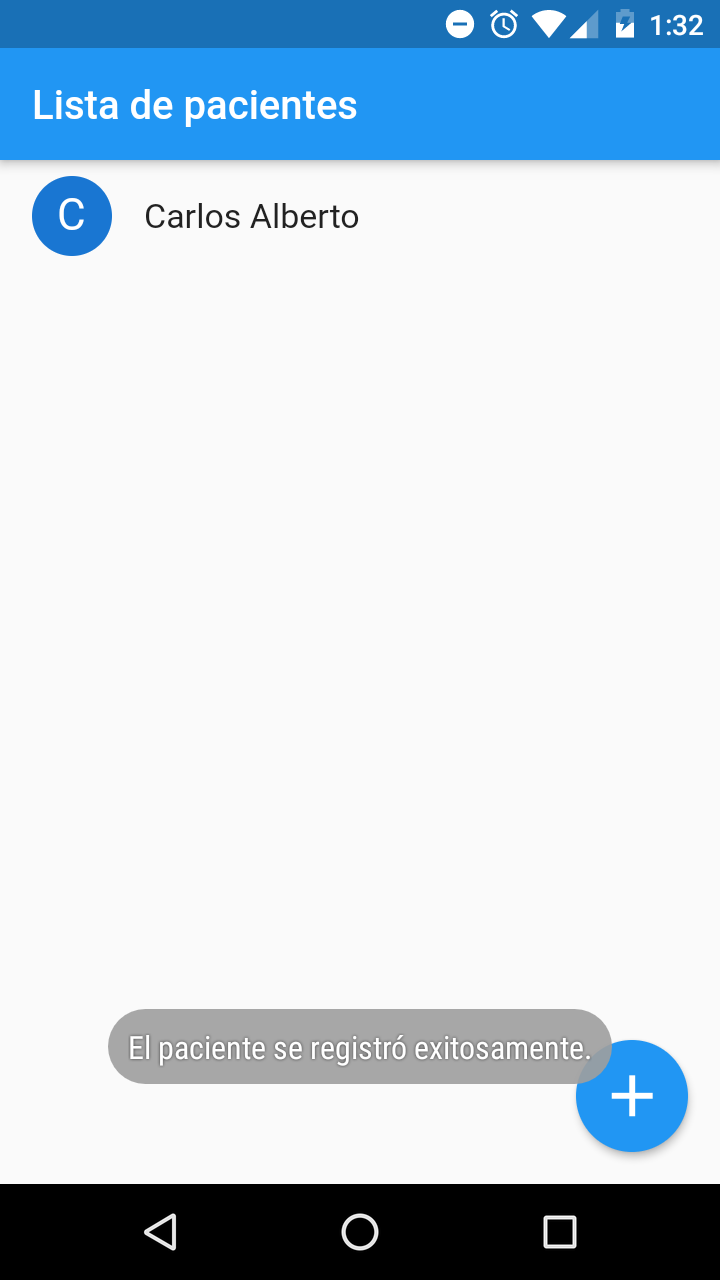
\includegraphics[width=0.5\textwidth]{AvancesPruebas/imagenes/app/ui_regExitoso.png}}
		\caption{IU Consultar pacientes \label{fig:casosUso:resumenUI1}}
	\end{center}
\end{figure}


\subsubsection{IU Registrar paciente}
La figura \ref{fig:casosUso:resumenUI2} muestra la pantalla ''Registrar paciente'', en la cual el usuario podrá ingresar los datos del paciente (Nombre, Teléfono, Fecha de nacimiento y Sexo). Con el teléfono registrado en esta pantalla se realizará la búsqueda de los mensajes para recuperar la información de las mediciones.

\begin{figure}[htpb!]
	\begin{center}
		\fbox{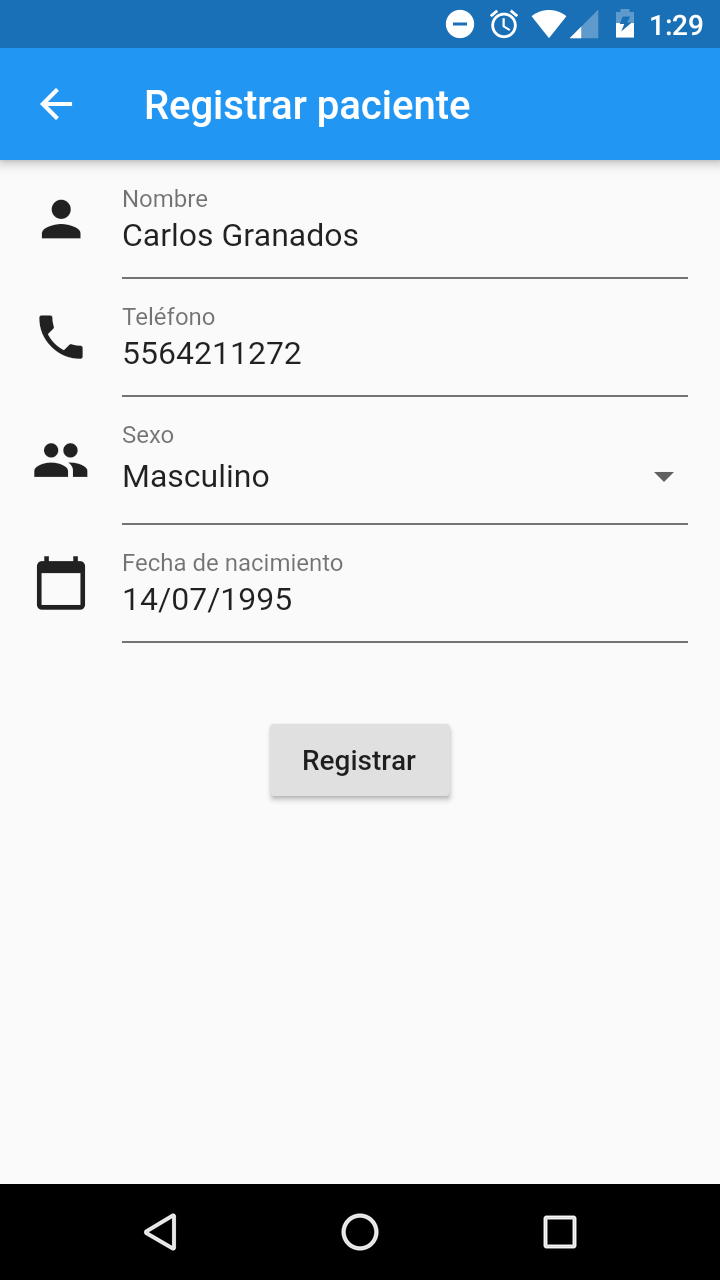
\includegraphics[width=0.5\textwidth]{AvancesPruebas/imagenes/app/ui_registroDatos.png}}
		\caption{IU Registrar paciente \label{fig:casosUso:resumenUI2}}
	\end{center}
\end{figure}


\subsubsection{IU Consultar información del paciente}
La figura \ref{fig:casosUso:resumenUI3} muestra la pantalla ''Consultar información del paciente'', en la que se muestra la sección Información general del paciente con el teléfono, sexo y edad calculada con la fecha de nacimiento registrada. Además de un promedio de mediciones en la que se calcula el promedio de la temperatura y la frecuencia cardíaca obtenidos a partir de todas las mediciones registradas.

\begin{figure}[htpb!]
	\begin{center}
		\fbox{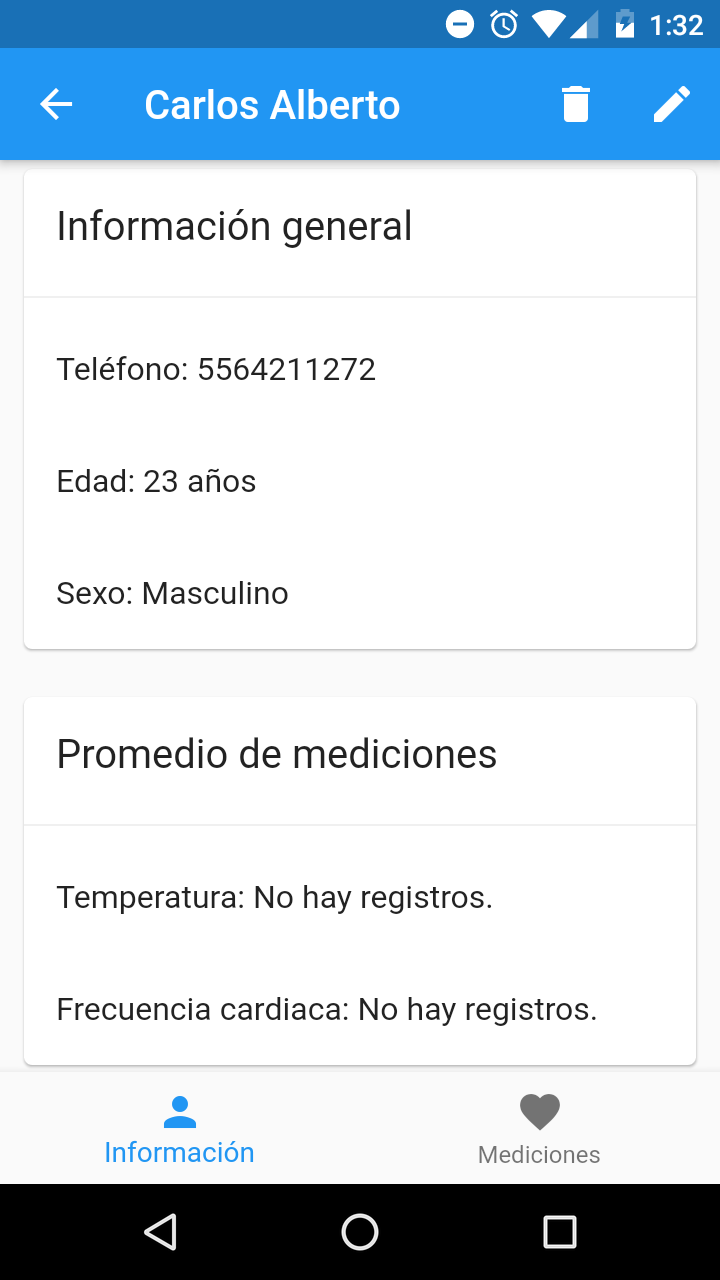
\includegraphics[width=0.5\textwidth]{AvancesPruebas/imagenes/app/ui_info.png}}
		\caption{IU Consultar información del paciente \label{fig:casosUso:resumenUI3}}
	\end{center}
\end{figure}


\subsubsection{IU Editar información del paciente}
La figura \ref{fig:casosUso:resumenUI4} muestra la pantalla ''Editar información del paciente'', en la cual el usuario podrá modificar los datos del paciente (Nombre, Teléfono, Fecha de nacimiento y Sexo).

\begin{figure}[htpb!]
	\begin{center}
		\fbox{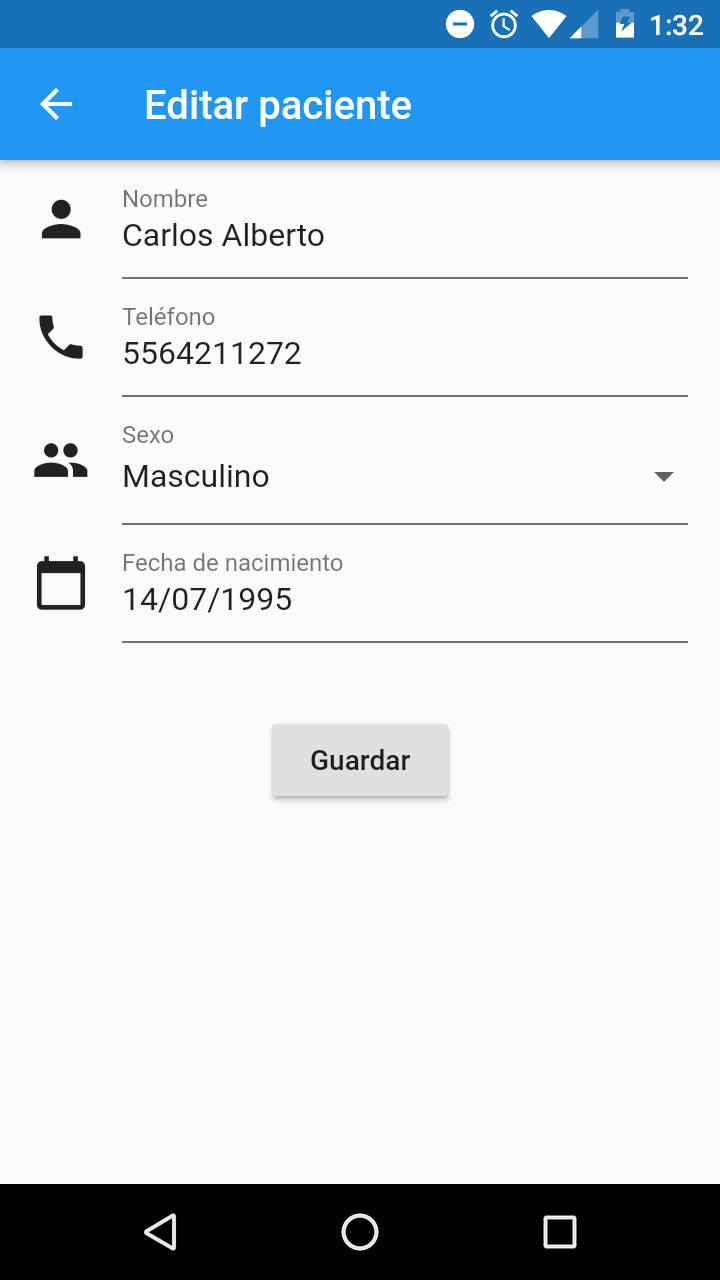
\includegraphics[width=0.5\textwidth]{AvancesPruebas/imagenes/app/ui_editar.png}}
		\caption{IU Consultar información del paciente \label{fig:casosUso:resumenUI4}}
	\end{center}
\end{figure}


\subsubsection{IU Consultar registros de signos vitales}
La figura \ref{fig:casosUso:resumenUI5} muestra la pantalla ''Consultar registros de signos vitales'', en la cual el usuario podrá visualizar todas las mediciones registradas, con la información recuperada de los mensajes enviados desde el sistema embebido.

\begin{figure}[htpb!]
	\begin{center}
		\fbox{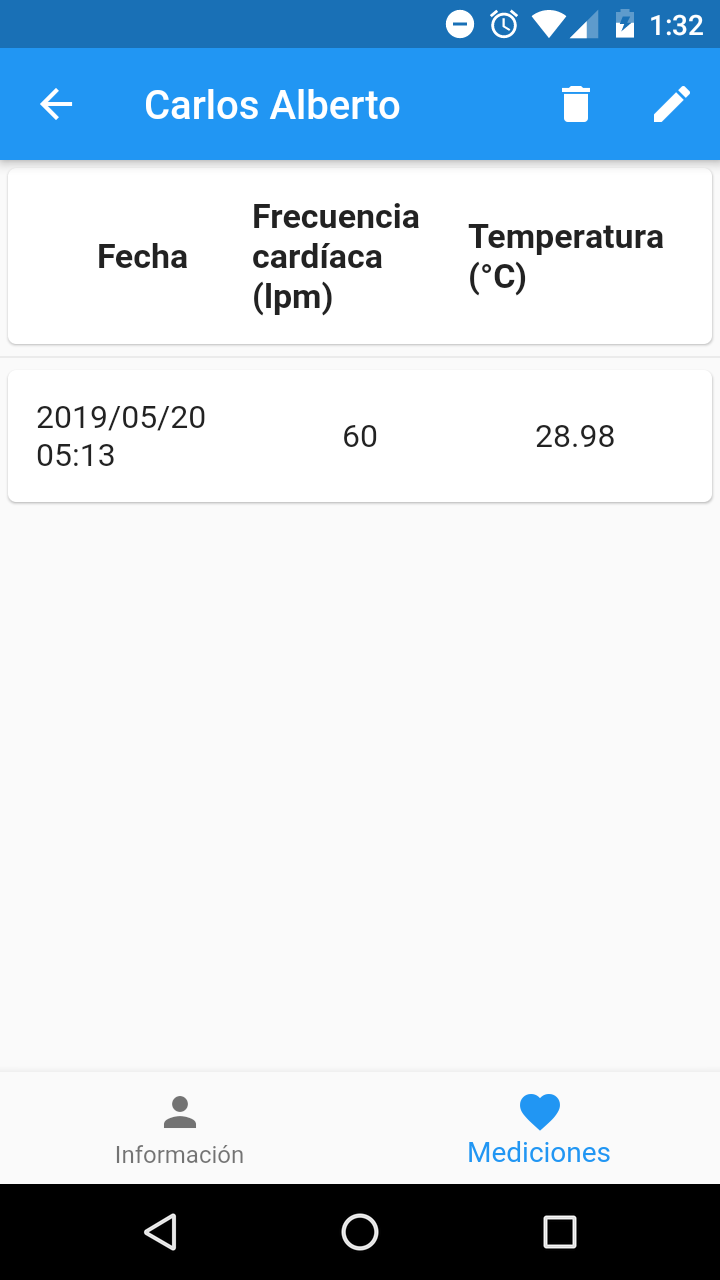
\includegraphics[width=0.5\textwidth]{AvancesPruebas/imagenes/app/ui_medicion.png}}
		\caption{IU Consultar registros de signos vitales\label{fig:casosUso:resumenUI5}}
	\end{center}
\end{figure}
